\chapter{Comparaison entre Gadget et un code Vlasov\label{Chap::VlasovGadget}}
	\minitoc%

	\todo[inline]{Ce chapitre en est à peine à son premier jet. Toutes les figures ne sont pas encore commenté (ça arrivera dans le courant de la
	semaine). Il manque aussi les figures contenant tous les $j$ sommé.}

	% Une des questions qui se posent avec notre approche concerne sa validité. En effet, à quel point gadget peut il
	% être proche d'un programme résolvant directement les équations de Vlasov-Poisson. Dans ce chapitre, nous tentons
	% d'apporter des éléments de réponse.

	Avant de présenter les résultats obtenus au cours de la thèse, nous allons présenter un travail que nous avons effectué en parallèle. Il a été
	effectué conjointement avec Stéphane Colombi, Thierry Sousbie et Sébastien Peirani. Il consiste à comparer les résultats donnés par un code
	résolvant numériquement l'équation de Vlasov (écrit par Thierry Sousbie en se basant sur~\cite{1983PASJ...35..547F}) et le code $N$-corps
	\textsc{gadget-2}.

	\section{Description du code Vlasov}

		Nous considérons un système à symétrie sphérique . L'équation de Vlasov s'écrit:
		\begin{align}
			\pderivn{f}{t} + v_r\pderivn{f}{r} + \(\dfrac{j^2}{r^3} - \dfrac{GM(r)}{r^2}\)\pderivn{f}{v_r} = 0\label{Eq::ValGad::Pois}
		\end{align}
		avec $f = f(r, u, j, t)$ la fonction de distribution dans l'espace des phases du système au temps $t$, $r$ le rayon de l'objet, $v_r$
		la vitesse radiale et $j$ le moment angulaire. La fonction $M(r)$ donne la masse contenu à l'intérieur de la sphère de rayon $r$.

		Pour résoudre l'équation, l'espace des phases $\(r, v_r, j\)$ est discrétisé sur un maillage tridimensionnel de dimension $(r, v_r,
		j)\in\(\left[r_\mathrm{min}; r_\mathrm{max}\right], \left[-v_r^\mathrm{max}; v_r^\mathrm{max}\right], \left[0;
		j_\mathrm{max}\right]\)$ avec $r$ évoluant logarithmiquement.
		Chaque point du maillage
		est considéré comme une particule. L'équation~\ref{Eq::ValGad::Pois} est séparée en deux opérateurs:
		\begin{itemize}
			\item un premier opérateur qui nous permet d'obtenir la trajectoire d'une particule libre:
				\begin{align*}
					\pderivn{f}{t} + v_r\pderivn{f}{r} + \dfrac{j^2}{r^3}\pderivn{f}{u} = 0
				\end{align*}
			\item un second permettant de calculer l'accélération:
				\begin{align*}
					\pderivn{f}{t} - \dfrac{GM(r)}{r^2}\pderivn{f}{v_r} = 0
				\end{align*}
		\end{itemize}
		Ces deux opérateurs, allié à un schéma de type \og{}Leap-frog\fg, vont nous permettre de faire évoluer chaque point du maillage du
		temps $t$ au temps $t+dt$. Puis, en utilisant le fait que chaque couche de moment angulaire sont indépendantes les unes des autres,
		une interpolation de la fonction de distribution dans le plan $\(r, v_r\)$ pour chaque $j$ permet de reconstruire le maillage.

		L'axe selon $r$ évoluant logarithmiquement, un problème va se poser lorsque $r\to0$. Pour l'éviter, il fait l'approximation que les
		particules à l'intérieur du rayon $r_\mathrm{min}$ sont libres. Il doit donc être suffisamment petit pour que cette approximation soit
		vérifié, mais suffisamment grand pour éviter la divergence du logarithme.
		% toutes les particules passant sous ce rayon $r_\mathrm{min}$ puissent évoluer comme des particules libres.

		Plus de détail sur le fonctionnement du code pourront être trouvé dans l'article associé à cette étude (référence?).
		Pour effectuer la comparaison de ce code à \textsc{gadget-2}, nous allons utiliser une sphère de Hénon de viriel $\gamma$. Dû à certaine
		limitation inhérente à l'interpolation, nous avons dû lissé cette sphére en multipliant la fonction de distribution par la fonction:
		\begin{align*}
			g(r) = \mathrm{erf}\( \dfrac{R - r }{ r_\epsilon }\) + 1
		\end{align*}
		où $R$ est le rayon de l'objet et $r_\epsilon$ le rayon sur lequel la sphère sera lissée.

		% Le code auquel nous allons comparer Gadget a été écrit par Thierry Sousbie et s'inspire grandement de
		% \citet{1983PASJ...35..547F}. Pour résoudre l'équation de Valsov, nous effectuons un changement de
		% coordonnées pour passer des positions-vitesses au jeu de variable utilisant la vitesse radiale
		% algébrique $u$, le rayon $r$ et le moment cinétique $j$. Ensuite, la fonction de distribution $f(r, u, j)$ est échantillonnée sur
		% un maillage cubique.

		% L'évolution de ce maillage se fait en considérant chaque point comme une particule libre. Le déplacement
		% de chaque particule se fait en décomposant l'équation de Vlasov en résolvant le système suivant pour:
		% \begin{align}
			% \begin{cases}
				% \dfrac{\partial f}{\partial t} + u\dfrac{\partial f}{\partial r} + \dfrac{j^2}{r^3}\dfrac{\partial f}{\partial u} = 0 \\
				% \\
				% \dfrac{\partial f}{\partial t} - \dfrac{GM_r}{r^2}\dfrac{\partial f}{\partial u} = 0
			% \end{cases} \label{Eq::VlasovGadget::EvoMaillage}
			% \intertext{avec:}
			% M_r = \int_0^r 4\pi r^2\rho(r)\mathrm{dr} \notag
			% \intertext{et}
			% \rho(r, t) = r^{-2}\int_0^\infty\mathrm{dj}2\pi j\int_{-\infty}^\infty\mathrm{du}f(r, u, j, t) \notag
		% \end{align}
		% Chaque équation du système est résolue pour un demi pas de temps l'une après l'autre.
		% La première équation du système~\ref{Eq::VlasovGadget::EvoMaillage} donne le mouvement libre d'une
		% particule tandis que la seconde donne l'accélération s'appliquant à cette dernière.
		% Ensuite, pour porter les modifications des positions des particules à la grille, une interpolation,
		% faîte à l'aide de spline, est utilisée.

		% Au niveau de l'échantillonnage, s'il est simple au niveau des vitesses et du moment cinétique, le rayon
		% pose plusieurs soucis. En effet, du fait des grandes valeurs autorisé et de la volonté des gens d'avoir
		% une bonne résolution au centre, il est impératif d'utiliser une échelle logarithmique: il n'est donc pas
		% possible d'aller jusqu'à $r=0$, il faut descendre jusqu'à $r=R_\mathrm{min}$. Pour modéliser ce qui se
		% passe dans l'intervalle $\left[0; R_\mathrm{min}\right]$, le code utilise un \og kernel\fg. Dans ce
		% kernel, le mouvement des particules est simulé en considérant qu'elles se déplacent sans qu'aucune
		% force ne s'applique. Il faut donc choisir $R_\mathrm{min}$ de sorte à ce que cette hypothèse soit vrai.

		% Une limite du code, venant des interpolations, c'est que les discontinuités du profil doivent être
		% lissées.
		% Nous allons donc utiliser une sphère de Hénon légèrement modifié: nous multiplions la fonction de
		% distribution par la fonction:
		% \begin{align*}
			% g(r) = \mathrm{erf}\( \dfrac{r_\mathrm{max} - r }{ r_\epsilon }\) + 1
		% \end{align*}
		% où $r_\mathrm{max}$ est le rayon de l'objet, $r_\epsilon$ le rayon sur lequel la sphère sera lissée.

		Dans la section suivante, nous allons comparer l'évolution de la sphère de Hénon avec un viriel de $\gamma=-0,5$ puis nous
		enchaînerons sur une comparaison utilisant un viriel de $\gamma=-0.1$.

	\section{Comparaison pour $\gamma = -0.5$}

		Nous allons commencer par comparer nos deux codes numériques pour des conditions initiales dont l'évolution est bien connu et décrite
		dans la littérature: nous allons regarder l'effondrement d'une sphère de Hénon de viriel $\gamma=-0,5$. Nous prenons comme référence
		l'article de~\cite{1983PASJ...35..547F}. Nous nous placerons dans le même système d'unités.

		Pour comparer nos simulations, nous nous baserons sur la correspondance entre l'espace des phases $(r, v_r)$ pour $j=0,425$ et
		l'évolution du profil de densité de l'objet. Nous effectuerons ces comparaison à différent temps afin de montrer que nous obtenons
		bien le même comportement au cours du temps. La simulation \textsc{gadget-2} utilisée ici comporte $10^6$ particules. L'article
		associé étudiera aussi l'évolution de simulations composées de $10^5$ et $10^7$ particules.

		\todo[inline]{L'impact du lissage de la force. À rédiger selon ce qui est dit dans l'article. Pas possible de présenter l'étude sur le pas de temps,
		je n'ai rien d'utilisable.}
		% \begin{figure}[htbp]
			% \begin{subfigure}{0.5\linewidth}
				% \centering 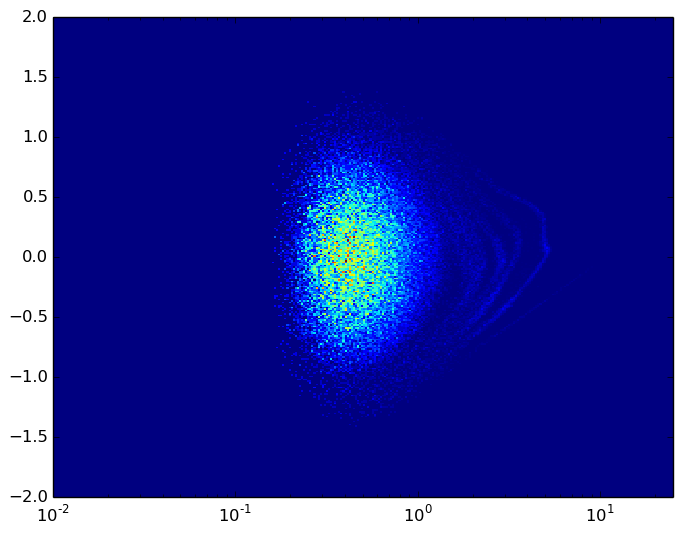
\includegraphics[width=\linewidth]{{vlasov_gadget/Vlasov_0.5_Soft/smoothed_0.5_045_0.00001_phasespace}.png}
				% \caption{Représentation de l'espace des phase à $j=0.425$ et $t=45$ pour $\gamma=-0,5$ et
					% $\epsilon=0.00001$.\label{Fig::ValGad::0.5::Soft1}}
			% \end{subfigure}\hfill
			% \begin{subfigure}{0.5\linewidth}
				% \centering 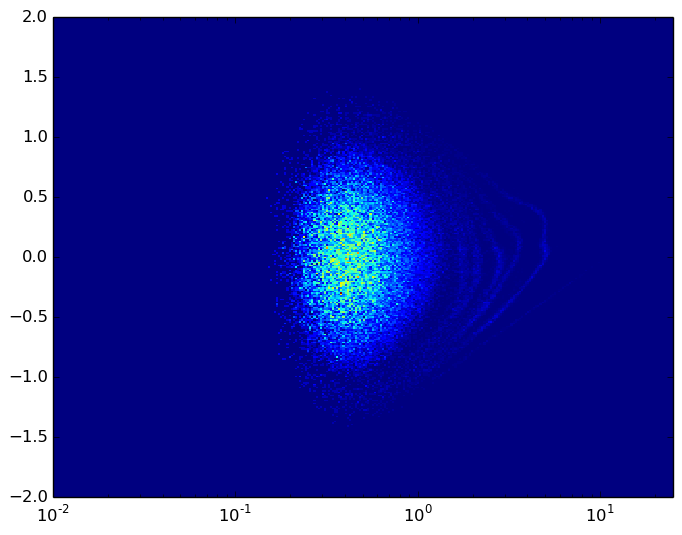
\includegraphics[width=\linewidth]{{vlasov_gadget/Vlasov_0.5_Soft/smoothed_0.5_045_0.0001_phasespace}.png}
				% \caption{Représentation de l'espace des phase à $j=0.425$ et $t=45$ pour $\gamma=-0,5$ et
					% $\epsilon=0.00001$.\label{Fig::ValGad::0.5::Soft2}}
			% \end{subfigure}
			% \begin{subfigure}{0.5\linewidth}
				% \centering 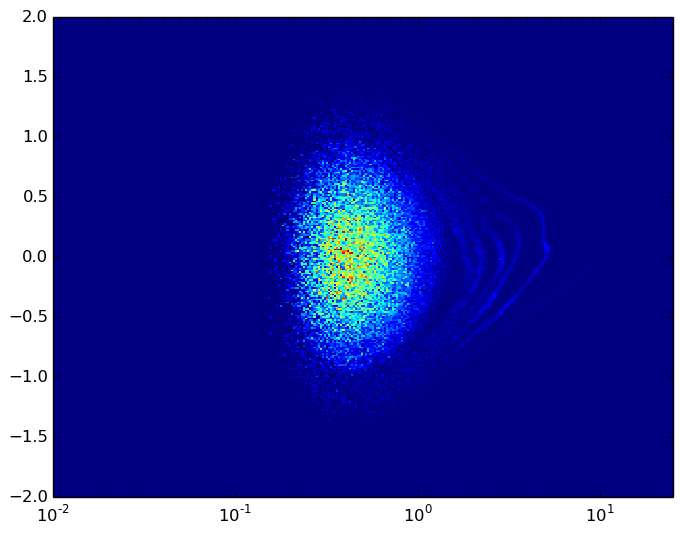
\includegraphics[width=\linewidth]{{vlasov_gadget/Vlasov_0.5_Soft/smoothed_0.5_045_0.01_phasespace}.png}
				% \caption{Représentation de l'espace des phase à $j=0.425$ et $t=45$ pour $\gamma=-0,5$ et
					% $\epsilon=0.00001$.\label{Fig::ValGad::0.5::Soft3}}
			% \end{subfigure}\hfill
			% \begin{subfigure}{0.5\linewidth}
				% \centering 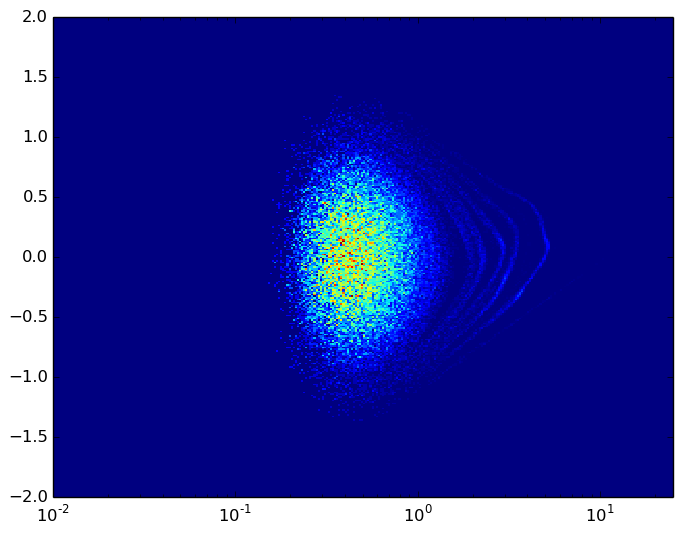
\includegraphics[width=\linewidth]{{vlasov_gadget/Vlasov_0.5_Soft/smoothed_0.5_045_0.1_phasespace}.png}
				% \caption{Représentation de l'espace des phase à $j=0.425$ et $t=45$ pour $\gamma=-0,5$ et
					% $\epsilon=0.00001$.\label{Fig::ValGad::0.5::Soft4}}
			% \end{subfigure}
		% \end{figure}

		Le premier temps que nous regardons est $t=0$. La figure~\ref{Fig::ValGad::0.5::t0} montre l'espace des phases pour les conditions
		initiales. La première chose à noter concerne la différence apparente concernant le maximum de la fonction de distributions. Cette
		différence est dû au faible nombre de particules présentes dans la couche de $j$ choisi. Excepté ce point, nous retrouvons bien la
		croissance progressive du nombre de particule ainsi qu'un étalement progressif des vitesses radiales quand $r$ augmente.
		\begin{figure}[htbp]
			\centering \includegraphics[width=\linewidth]{{CompVlasGad_t_0_512_0.5}.png}
			\caption{Comparaison de l'espace des phases entre le code vlasov (à gauche) et le code Gadget (à droite), à $t=0$ et pour $j=0.425$.\label{Fig::ValGad::0.5::t0}}
		\end{figure}
		Du côté du profil de densité (figure~\ref{Fig::ValGad::0.5::Density::t0}), l'accord est très bon, excepté au centre du système où le manque de particules empêche le calcul précis
		de la densité.
		\begin{figure}[htpb]
			\centering \includegraphics{{CompVlasGad_Density_0.5_t_0_error}.pdf}
			\caption{Comparaison du profil de densité entre le code vlasov (en bleu) et le code gadget (en vert), pour $t=0$.\label{Fig::ValGad::0.5::Density::t0}}
		\end{figure}

		Le deuxième temps que nous avons choisi de montrer se situe peu après la fin de l'effondrement de la sphère de Hénon. Le nombre
		d'enroulement présent sur les graphiques de la figure~\ref{Fig::ValGad::0.5::t13} sont les mêmes. Par contre, l'enroulement central
		donne de la simulation gadget semble un peu en avance sur la simulation vlasov. Ce qui semble confirmé par le \og{}bras\fg s'étendant
		jusqu'à $r=3$ pour la simulation vlasov et jusqu'à $r=4$ pour la simulation gadget.
		\begin{figure}[htbp]
			\centering \includegraphics[width=\linewidth]{{CompVlasGad_t_13_512_0.5}.png}
			\caption{Comparaison de l'espace des phases entre le code vlasov (à gauche) et le code Gadget (à droite), à $t=13$ et pour $j=0.425$.\label{Fig::ValGad::0.5::t13}}
		\end{figure}
		Les profils de densité présenté sur la figure~\ref{Fig::ValGad::0.5::Density::t13} montre par contre un très bon accord, excepté au
		bord du système, où le nombre de particules recommence alors à faiblir. L'extension du système en $r$ est aussi visible.
		\begin{figure}[htpb]
			\centering \includegraphics{{CompVlasGad_Density_0.5_t_13_error}.pdf}
			\caption{Comparaison du profil de densité entre le code vlasov (en bleu) et le code gadget (en vert), pour $t=13$.\label{Fig::ValGad::0.5::Density::t13}}
		\end{figure}
		Cette extension du profil peut-être expliqué par l'éjection d'une fraction des particules hors du système suite aux collisions se
		produisant dans le système.

		Pour terminer la comparaison à ce viriel, nous regardons ce qu'il se passe à $t=45$. À ce moment, le système a eu le temps de se
		stabiliser. Nous remarquons, en regardant la figure~\ref{Fig::ValGad::0.5::t45}, que la simulation gadget présente des
		\og{}vaguelettes\fg sur les enroulements extérieurs qui semble en avance sur la simulation vlasov.
		\begin{figure}[htbp]
			\centering \includegraphics[width=\linewidth]{{CompVlasGad_t_45_512_0.5}.png}
			\caption{Comparaison de l'espace des phases entre le code vlasov (à gauche) et le code Gadget (à droite), à $t=45$ et pour $j=0.425$.\label{Fig::ValGad::0.5::t45}}
		\end{figure}
		\begin{figure}[htpb]
			\centering \includegraphics{{CompVlasGad_Density_0.5_t_45_error}.pdf}
			\caption{Comparaison du profil de densité entre le code vlasov (en bleu) et le code gadget (en vert), pour $t=45$.\label{Fig::ValGad::0.5::Density::t45}}
		\end{figure}


	\section{Comparaison pour $\gamma = -0.1$}

		Nous allons commencer par comparer nos deux codes numériques pour des conditions initiales dont l'évolution est bien connu et décrite
		dans la littérature: nous allons regarder l'effondrement d'une sphère de Hénon de viriel $\gamma=-0,5$. Nous prenons comme référence
		l'article de~\cite{1983PASJ...35..547F}. Nous nous placerons dans le même système d'unités.

		Pour comparer nos simulations, nous nous baserons sur la correspondance entre l'espace des phases $(r, v_r)$ pour $j=0,425$ et
		l'évolution du profil de densité de l'objet. Nous effectuerons ces comparaison à différent temps afin de montrer que nous obtenons
		bien le même comportement au cours du temps. La simulation \textsc{gadget-2} utilisée ici comporte $10^6$ particules. L'article
		associé étudiera aussi l'évolution de simulations composées de $10^5$ et $10^7$ particules.

		Le premier temps que nous regardons est $t=0$. La figure~\ref{Fig::ValGad::0.1::t0} montre l'espace des phases pour les conditions
		initiales. La première chose à noter concerne la différence apparente concernant le maximum de la fonction de distributions. Cette
		différence est dû au faible nombre de particules présentes dans la couche de $j$ choisi. Excepté ce point, nous retrouvons bien la
		croissance progressive du nombre de particule ainsi qu'un étalement progressif des vitesses radiales quand $r$ augmente.
		\begin{figure}[htbp]
			\centering \includegraphics[width=\linewidth]{{CompVlasGad_t_0_512_0.1}.png}
			\caption{Comparaison de l'espace des phases entre le code vlasov (à gauche) et le code Gadget (à droite), à $t=0$ et pour $j=0.425$.\label{Fig::ValGad::0.1::t0}}
		\end{figure}
		Du côté du profil de densité (figure~\ref{Fig::ValGad::0.1::Density::t0}), l'accord est très bon, excepté au centre du système où le manque de particules empêche le calcul précis
		de la densité.
		\begin{figure}[htpb]
			\centering \includegraphics{{CompVlasGad_Density_0.1_t_0}.pdf}
			\caption{Comparaison du profil de densité entre le code vlasov (en bleu) et le code gadget (en vert), pour $t=0$.\label{Fig::ValGad::0.1::Density::t0}}
		\end{figure}

		Le deuxième temps que nous avons choisi de montrer se situe peu après la fin de l'effondrement de la sphère de Hénon. Le nombre
		d'enroulement présent sur les graphiques de la figure~\ref{Fig::ValGad::0.1::t5} sont les mêmes. Par contre, l'enroulement central
		donne de la simulation gadget semble un peu en avance sur la simulation vlasov. Ce qui semble confirmé par le \og{}bras\fg s'étendant
		jusqu'à $r=3$ pour la simulation vlasov et jusqu'à $r=4$ pour la simulation gadget.
		\begin{figure}[htbp]
			\centering \includegraphics[width=\linewidth]{{CompVlasGad_t_5_512_0.1}.png}
			\caption{Comparaison de l'espace des phases entre le code vlasov (à gauche) et le code Gadget (à droite), à $t=5$ et pour $j=0.425$.\label{Fig::ValGad::0.1::t5}}
		\end{figure}
		Les profils de densité présenté sur la figure~\ref{Fig::ValGad::0.1::Density::t5} montre par contre un très bon accord, excepté au
		bord du système, où le nombre de particules recommence alors à faiblir. L'extension du système en $r$ est aussi visible.
		\begin{figure}[htpb]
			\centering \includegraphics{{CompVlasGad_Density_0.1_t_5}.pdf}
			\caption{Comparaison du profil de densité entre le code vlasov (en bleu) et le code gadget (en vert), pour $t=5$.\label{Fig::ValGad::0.1::Density::t5}}
		\end{figure}
		Cette extension du profil peut-être expliqué par l'éjection d'une fraction des particules hors du système suite aux collisions se
		produisant dans le système.

		Pour terminer la comparaison à ce viriel, nous regardons ce qu'il se passe à $t=45$. À ce temps, le système a eu le temps de se
		stabiliser après l'effondrement.
		\begin{figure}[htbp]
			\centering \includegraphics[width=\linewidth]{{CompVlasGad_t_25_512_0.1}.png}
			\caption{Comparaison de l'espace des phases entre le code vlasov (à gauche) et le code Gadget (à droite), à $t=25$ et pour $j=0.425$.\label{Fig::ValGad::0.1::t25}}
		\end{figure}
		\begin{figure}[htpb]
			\centering \includegraphics{{CompVlasGad_Density_0.1_t_25}.pdf}
			\caption{Comparaison du profil de densité entre le code vlasov (en bleu) et le code gadget (en vert), pour $t=25$.\label{Fig::ValGad::0.1::Density::t25}}
		\end{figure}

		\begin{figure}[htbp]
			\centering \includegraphics[width=\linewidth]{{CompVlasGad_t_35_512_0.1}.png}
			\caption{Comparaison de l'espace des phases entre le code vlasov (à gauche) et le code Gadget (à droite), à $t=35$ et pour $j=0.425$.\label{Fig::ValGad::0.1::t35}}
		\end{figure}
		\begin{figure}[htpb]
			\centering \includegraphics{{CompVlasGad_Density_0.1_t_35}.pdf}
			\caption{Comparaison du profil de densité entre le code vlasov (en bleu) et le code gadget (en vert), pour $t=35$.\label{Fig::ValGad::0.1::Density::t35}}
		\end{figure}
